\chapstart
\section{THIẾT KẾ GIAO DIỆN}
\subsection{Tổng quan về thiết kế giao diện}
Giao diện BroomSharing sử dụng xanh lục, xanh ngọc làm điểm nhấn trên nền trắng và xám nhẹ. Các màn hình thống nhất cách bố trí tiêu đề, trường nhập, thẻ thông tin và nút thao tác chính để làm nổi bật nội dung không gian.

Danh sách phòng sử dụng \texttt{RecyclerView} để tái sử dụng các View khi hiển thị dữ liệu \parencite{android_recycler}. Thanh điều hướng người thuê gồm Trang chủ, Bản đồ, Lượt thuê, Tin nhắn và Cá nhân; Host và Admin có khu vực quản lý riêng.

Bộ hình trong chương là prototype ban đầu do nhóm xây dựng trên Figma, thể hiện bố cục và hướng tương tác dự kiến. Các màn hình đặt trọng tâm vào trình tự sử dụng và cách nhóm thông tin; giao diện hiện thực cùng kết quả kiểm thử được trình bày ở các chương sau. Những lựa chọn xuất hiện trong prototype vì vậy được xem xét ở mức phương án thiết kế, không đồng nhất với toàn bộ chức năng đã tích hợp.

\subsubsection{Phân cấp thông tin và hành động}
Các màn hình tìm thuê được tổ chức theo mức độ cần thiết của thông tin. Trang chủ ưu tiên ảnh, loại không gian và giá để hỗ trợ so sánh; chi tiết phòng bổ sung điều kiện sử dụng và vị trí; bước xác nhận tập hợp thời gian, liên hệ và chi phí trước khi gửi yêu cầu. Dữ liệu được mở dần theo tiến trình, tránh đặt toàn bộ nội dung của phòng lên thẻ danh sách.

Hành động chính sử dụng màu nhấn và tên gắn với mục tiêu như đăng nhập, thuê ngay hoặc gửi yêu cầu. Những thao tác phụ như xem lại, thay đổi thông tin và quay về được đặt gần khối liên quan. Đối với hủy, từ chối hoặc khóa đối tượng, thiết kế cần thể hiện rõ đích tác động và bước xác nhận, vì các thao tác này làm thay đổi quyền sử dụng hoặc trạng thái xử lý.

\subsubsection{Trạng thái giao diện và tính nhất quán}
Thiết kế phân biệt đang tải, dữ liệu trống, dữ liệu không hợp lệ và kết quả gửi. Danh sách chưa tải xong không được thể hiện như không có kết quả; nút đã nhấn cũng chưa phải xác nhận lưu thành công. Khi gửi biểu mẫu, trạng thái xử lý giúp hạn chế thao tác lặp. Nếu có lỗi, thông báo gắn với nội dung cần sửa và giữ lại phần dữ liệu còn phù hợp. Các phản hồi này là yêu cầu cho bản hiện thực từ prototype.

\clearpage

\subsection{Giao diện phân hệ người thuê}
\subsubsection{Đăng nhập và đăng ký}
Giao diện đăng nhập gồm tài khoản, mật khẩu và đường dẫn đến đăng ký, quên mật khẩu. Màn hình đăng ký thu thập họ tên, thông tin liên hệ, mật khẩu và xác nhận mật khẩu. Các trường sắp theo thứ tự nhập, với điều khoản sử dụng đặt trước nút hoàn tất.

Hình~\ref{fig:ch3-auth} phân nhóm trường nhập và làm nổi bật nút đăng nhập, đăng ký. Biểu tượng mật khẩu hỗ trợ kiểm tra nội dung nhập; lựa chọn Google/Zalo đặt ở vùng riêng để phân biệt với biểu mẫu tài khoản của ứng dụng.

Khi biểu mẫu có lỗi, phản hồi cần phân biệt thiếu dữ liệu, thông tin chưa đúng định dạng và xác thực không thành công. Nội dung mật khẩu được che mặc định; dữ liệu còn hợp lệ không bị xóa chỉ vì một trường khác cần sửa. Liên kết giữa đăng nhập và đăng ký giữ vai trò điều hướng, không làm người dùng nhầm với nút gửi biểu mẫu hiện tại.

\begin{figure}[H]\centering
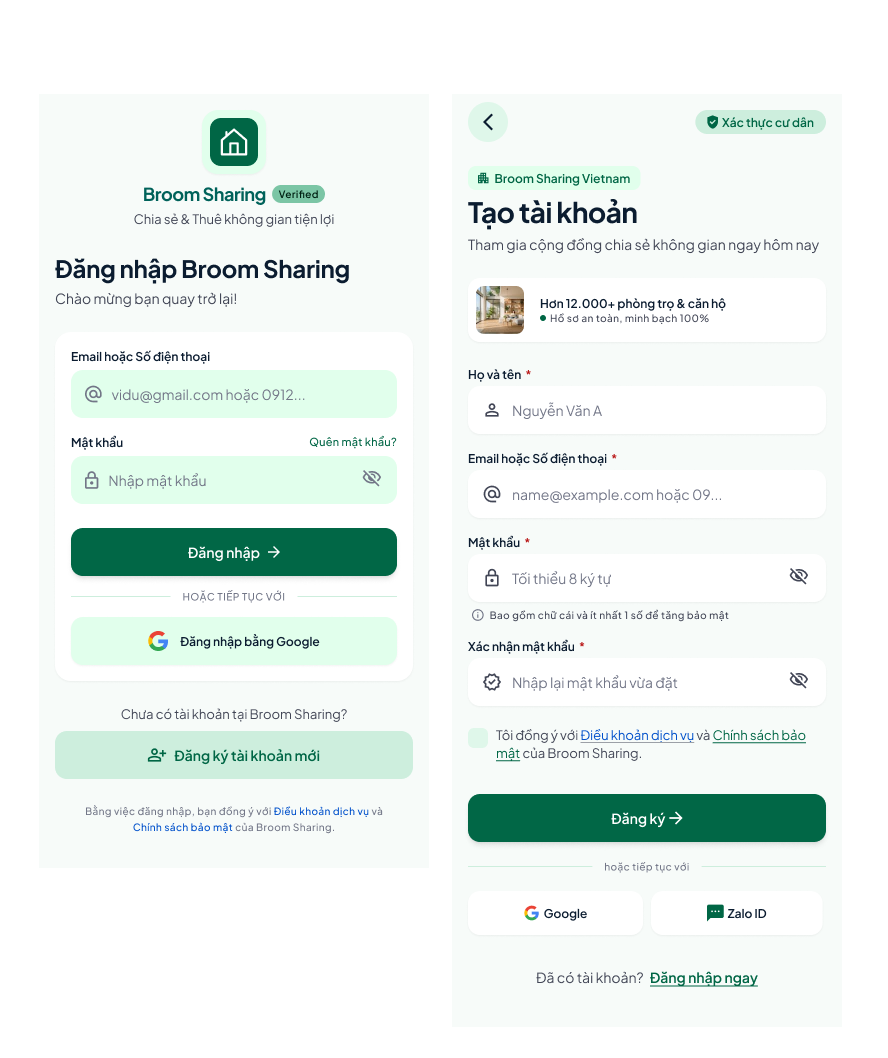
\includegraphics[width=0.9\textwidth,height=0.55\textheight,keepaspectratio]{chapter3/auth-design.png}
\caption{Thiết kế biểu mẫu đăng nhập và đăng ký tài khoản.}\label{fig:ch3-auth}
\end{figure}
\clearpage

\subsubsection{Trang chủ và chi tiết không gian}
Giao diện Trang chủ tích hợp thanh tìm kiếm, phân loại danh mục và danh sách không gian dưới dạng thẻ. Mỗi thẻ tập trung vào ảnh, tên phòng, khu vực, sức chứa và giá thuê. Hình~\ref{fig:ch3-home} minh họa thứ bậc hiển thị này qua hai vùng đối tác ưu tiên và không gian gợi ý. Thanh điều hướng đáy giữ các điểm truy cập chính ở vị trí ổn định khi duyệt danh sách.

Người dùng có thể tiếp cận bộ lọc từ vùng tìm kiếm và mở phòng cần xem. Màn hình chi tiết tại Hình~\ref{fig:ch3-detail} bổ sung bộ ảnh, diện tích, sức chứa, tiện ích, vị trí và thông tin Host. Nội dung dài được chia thành các khối để thuận tiện cuộn xem. Các hành động yêu thích, nhắn tin, chỉ đường và đặt thuê được bố trí gần thông tin liên quan để giảm thao tác chuyển màn hình.

Đơn vị giá cần đặt sát con số để phân biệt giá theo giờ với giá của kỳ thuê cố định. Các nhãn trạng thái và thông tin tiện ích giúp bổ sung ngữ cảnh, nhưng không thay thế phần điều kiện sử dụng trong chi tiết. Khi chuyển từ danh sách sang bản đồ hoặc mở phòng, lựa chọn phải tiếp tục trỏ đến cùng phòng để tránh nhầm đối tượng trước khi đặt.

\begin{figure}[H]\centering
\begin{minipage}[t]{0.31\textwidth}\centering
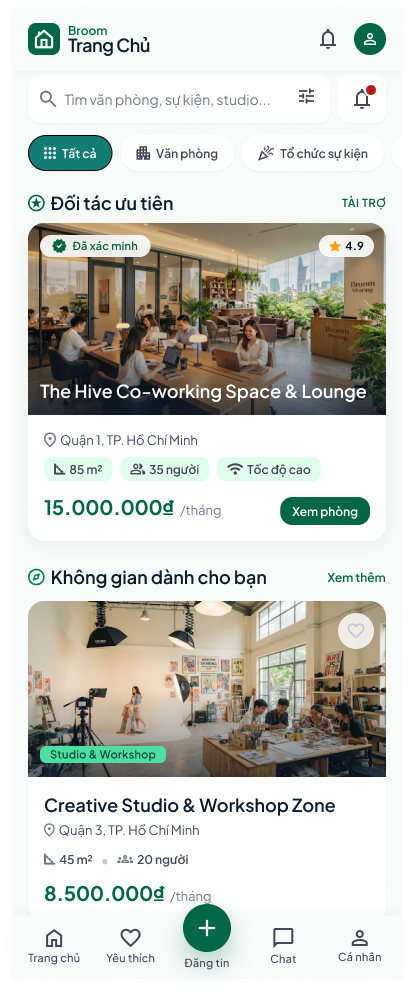
\includegraphics[width=\linewidth,height=0.47\textheight,keepaspectratio]{chapter3/home-design.png}
\caption{Thiết kế Trang chủ.}\label{fig:ch3-home}
\end{minipage}\hfill
\begin{minipage}[t]{0.65\textwidth}\centering
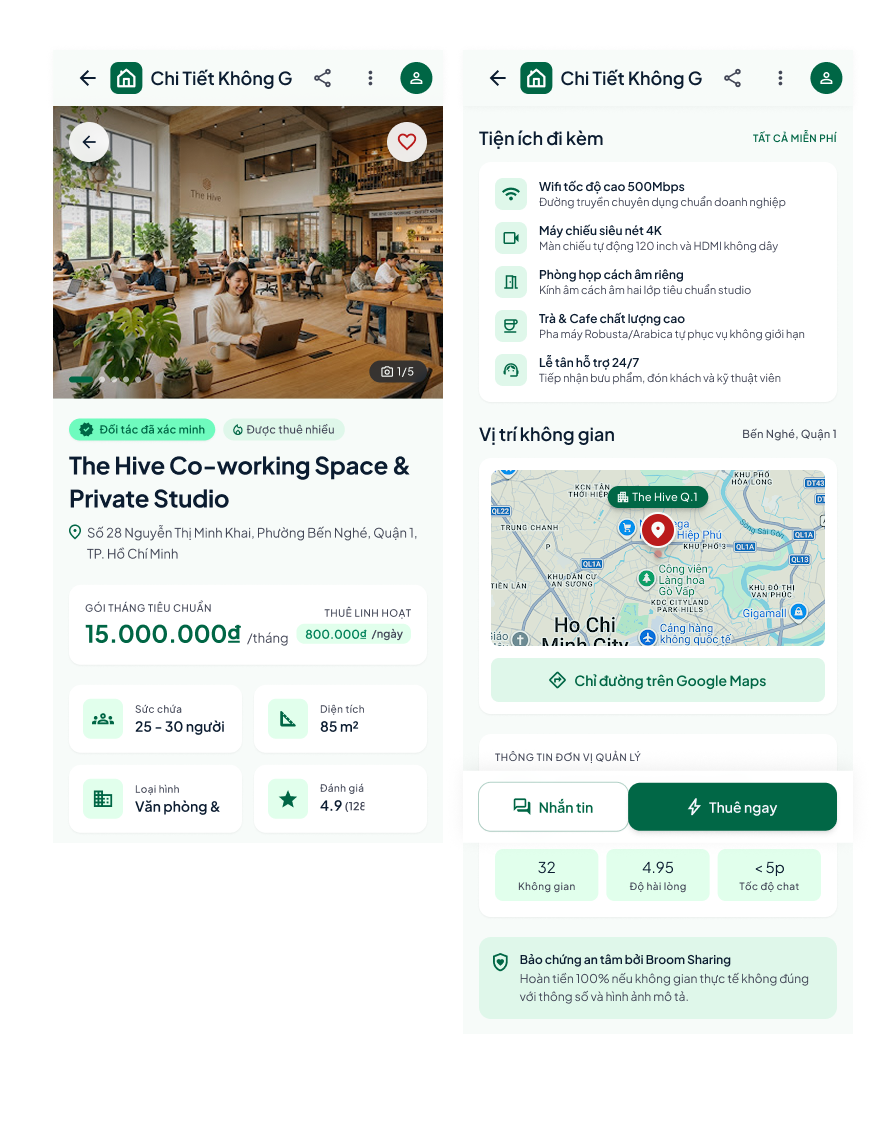
\includegraphics[trim=0 88 0 0,clip,width=\linewidth,height=0.47\textheight,keepaspectratio]{chapter3/detail-design.png}
\caption{Thiết kế thông tin chi tiết không gian.}\label{fig:ch3-detail}
\end{minipage}
\end{figure}

\clearpage
\subsubsection{Đặt chỗ, theo dõi và thanh toán}
Màn hình đặt chỗ tập hợp thời gian sử dụng, thông tin người thuê và giá dự kiến trước khi gửi yêu cầu. Khối thông tin phòng được giữ ở đầu màn hình để người dùng đối chiếu lựa chọn; vùng thời gian và liên hệ đặt ngay bên dưới. Đối với thiết kế nghiệp vụ, bộ chọn thời gian cần thích ứng với chế độ theo giờ hoặc kỳ thuê một, ba tháng của phòng.

Danh sách lượt thuê hiển thị thời gian, trạng thái booking và các thao tác còn hiệu lực. Phương án xác nhận tại Hình~\ref{fig:app-booking-design} tiếp tục chia nội dung thành hình thức thanh toán, thông tin hợp đồng và bảng chi phí. Tổng tiền cùng nút gửi yêu cầu nằm cuối tiến trình để người dùng kiểm tra trước khi xác nhận. Khi hiện thực luồng thanh toán, thông tin tiền cần tách khỏi trạng thái nhận phòng và hoàn tất.

Ở bước xác nhận, thay đổi kỳ thuê phải dẫn đến cập nhật phần thời gian và chi phí liên quan. Thiết kế dành vị trí cho thông tin người thuê, cho phép đối chiếu liên hệ mà không phải quay về hồ sơ để xem lại. Các nhãn bảo chứng, lựa chọn hợp đồng và số tiền cụ thể trong hình là nội dung minh họa của phương án ban đầu; thiết kế chi tiết khi triển khai phải bám chính sách đã xác định ở Chương 2.

\begin{figure}[H]\centering
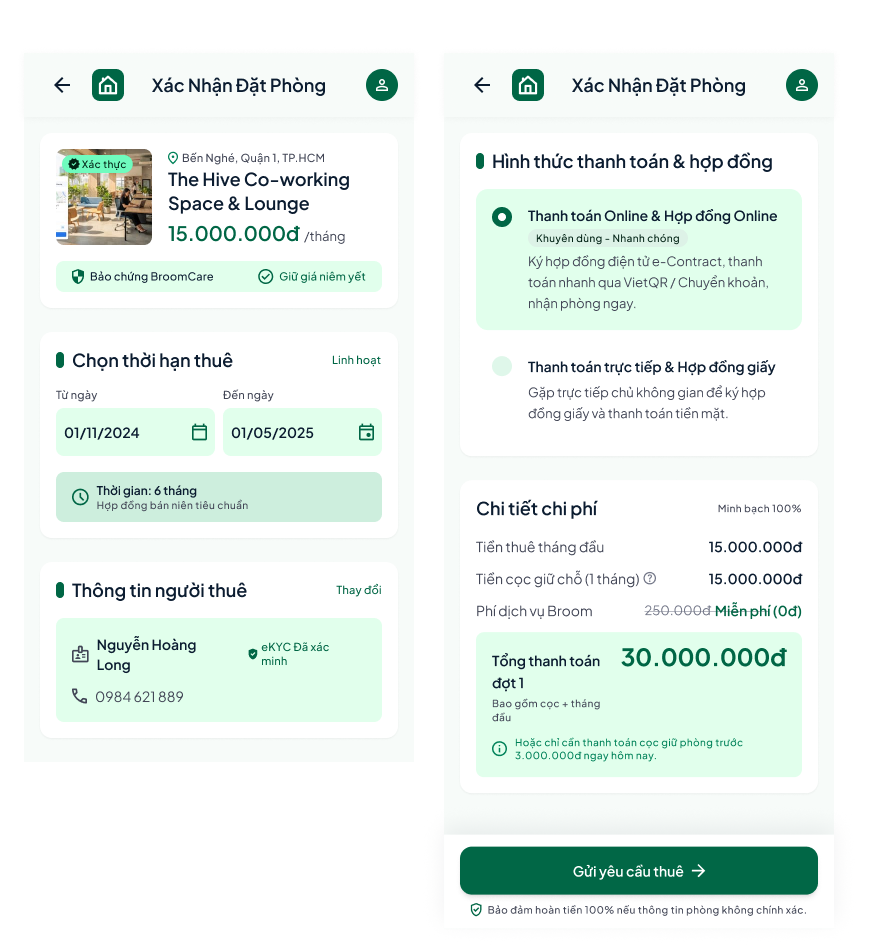
\includegraphics[width=\textwidth,height=0.48\textheight,keepaspectratio]{chapter3/booking-design.png}
\caption{Prototype xác nhận thông tin và chi phí đặt phòng.}\label{fig:app-booking-design}
\end{figure}

\clearpage
\subsubsection{Hồ sơ và tương tác}
Giao diện Cá nhân phân nhóm hồ sơ, ảnh đại diện, phòng yêu thích, lịch sử và đăng ký quyền Host. Khu vực tin nhắn tổ chức hội thoại với chủ không gian; hộp cập nhật tập trung sự kiện liên quan đến lượt thuê và trạng thái đã đọc.

Biểu mẫu đánh giá gồm điểm và nhận xét, chỉ mở sau lượt thuê đã xác nhận sử dụng và khép lại. Báo cáo vi phạm có nội dung riêng gửi Admin, tách khỏi nhận xét công khai về phòng.

Đối với hội thoại, danh sách cần thể hiện người trao đổi, nội dung gần nhất và tình trạng đã đọc; màn hình chat giữ ngữ cảnh phòng để hỗ trợ trao đổi. Thông tin chưa đọc phục vụ việc nhận biết thay đổi, không làm phát sinh một trạng thái mới của booking. Các đường dẫn từ thông báo hoặc hội thoại phải mở đúng đối tượng liên quan thay vì chỉ đưa về Trang chủ.

\subsection{Giao diện phân hệ chủ không gian}
Giao diện Host tập trung vào phòng, booking và lịch hoạt động. Khi đăng phòng, biểu mẫu phân nhóm thông tin cơ bản, giá và lịch, hình ảnh và điều kiện sử dụng. Hình~\ref{fig:ch3-host} minh họa cách giữ các trường cùng mục đích gần nhau trong ba bước nhập liệu.

Thông tin cơ bản gồm vị trí, loại không gian, diện tích và sức chứa. Phần giá và lịch tuân theo chế độ thuê của phòng; phần hình ảnh tập trung ảnh, mô tả và tiện ích. Thanh tiến trình cùng nút tiếp tục, quay lại giúp nhận biết bước hiện tại và kiểm tra thông tin trước khi gửi bài.

Tại màn hình booking, các thao tác của Host được phân biệt theo trạng thái: xác nhận, từ chối, hủy, nhận phòng, hoàn tất hoặc ghi nhận khách không đến. Những thao tác cần giải trình có ô nhập lý do. Màn hình lịch và danh sách phòng bổ sung góc nhìn tổng hợp về khoảng đã giữ, trạng thái bài đăng và yêu cầu cần xử lý.

Khi đăng tin theo nhiều bước, thông tin đã nhập cần được giữ trong quá trình đi tới hoặc quay lại giữa các bước của biểu mẫu. Vùng ảnh cần phân biệt ảnh đã chọn, đang tải và tải lỗi trước khi gửi bài. Đối với quản lý phòng, trạng thái chờ duyệt và trạng thái tạm ngừng không được thể hiện bằng cùng một nhãn, vì chúng có nguyên nhân và hành động tiếp theo khác nhau.

\begin{figure}[H]\centering
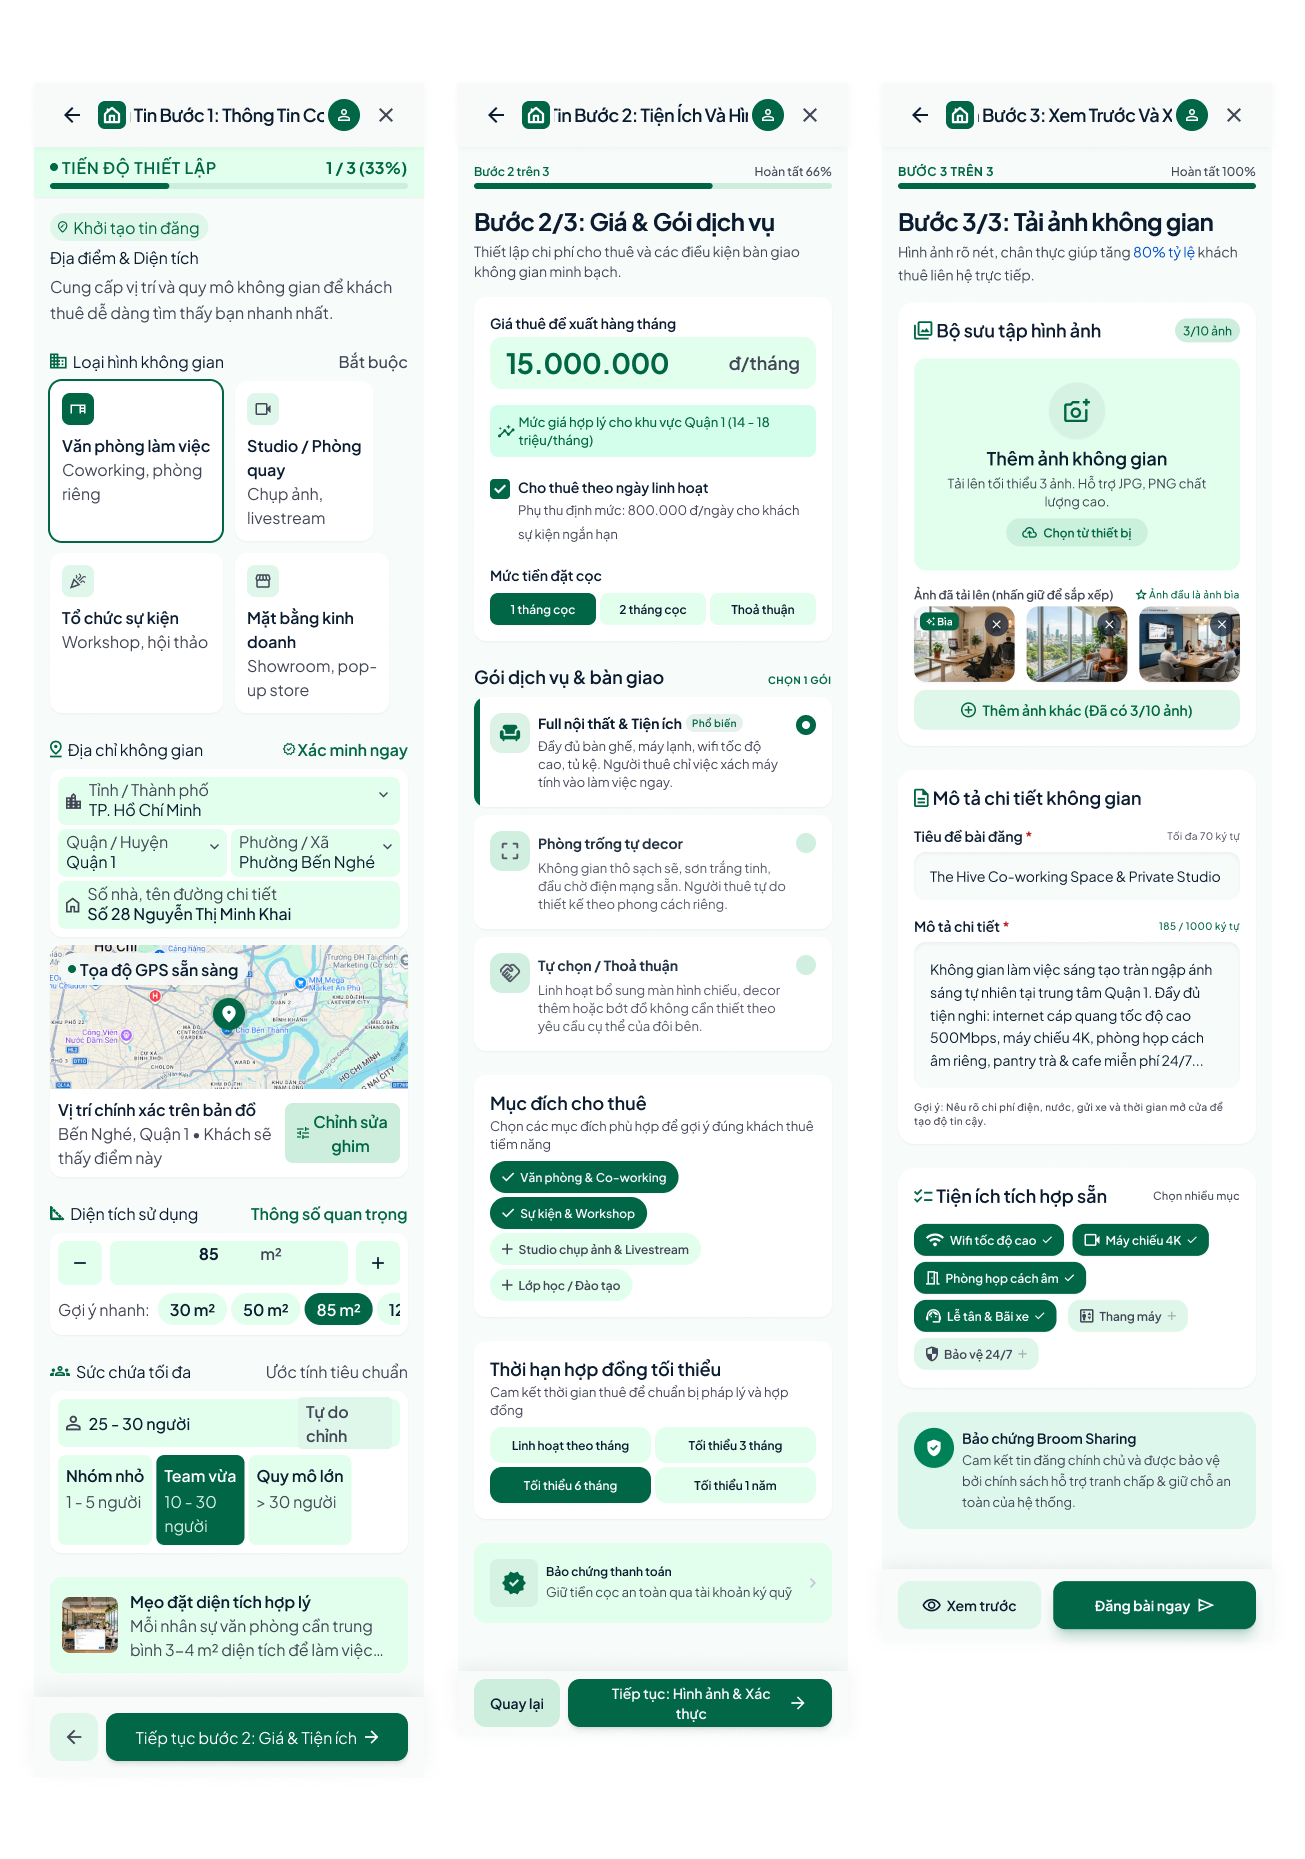
\includegraphics[width=\textwidth,height=0.5\textheight,keepaspectratio]{chapter3/host-design.png}
\caption{Prototype ba bước nhập thông tin và đăng không gian.}\label{fig:ch3-host}
\end{figure}

\subsection{Giao diện phân hệ quản trị viên}
Giao diện Admin phân chia khu vực tổng quan, xét duyệt, quản lý và báo cáo. Hồ sơ, bài đăng được hiển thị cùng trạng thái và mở chi tiết trước khi chấp thuận hoặc từ chối. Đơn xin quyền Host và minh chứng vị trí/hình ảnh là các nhóm độc lập.

Hình~\ref{fig:app-admin-design} đặt bộ lọc phía trên danh sách, gắn nút phê duyệt hoặc từ chối với hồ sơ đang xem. Trạng thái và lý do xử lý phân biệt khóa Host, đình chỉ phòng và khép booking. Các con số trong prototype phục vụ minh họa bố cục.

Trong thiết kế, danh sách cung cấp thông tin nhận diện nhanh, còn quyết định xử lý gắn với hồ sơ cụ thể. Trường hợp từ chối hoặc áp dụng hạn chế cần có vùng nhập lý do và xác nhận hành động. Hai nhóm kiểm duyệt phòng và quản lý tài khoản được bố trí riêng để phân biệt đối tượng chịu tác động; prototype đầy đủ được trình bày tại Phụ lục A.

